Analysis of experiments and results
\\
Building on the theory introduced in \ref{ch:point} and \ref{ch:prob}, this section covers the experiments carried out and the results obtained.

- Comments
\\
- Comparison
\\
- Table of loss scores
\\
Plots:
\\
- Plots for visualizing timeseries with quantiles bounds
\\
- Other plots that will come up to mind

\section{Point forecasting}
This section carries out a comparative study between the state of the art methods for point forecasting, introduced in \ref{ch:point}.
As use case, we will consider the task of predicting the load for the next month.
In such setting we have the following regressors
\begin{itemize}
    \item Day
    \item Hour
    \item Month
    \item Day of the week
    \item Is holiday
    \item Weather temperature
\end{itemize}
The metric upon we agreed is the root mean squared error, see section \ref{metrics}.
\subsection{Multiple linear regression}
To get started, standard multiple linear regression has been applied, see fig \ref{fig:mlr_price} for a visualisation. 
\begin{figure}
    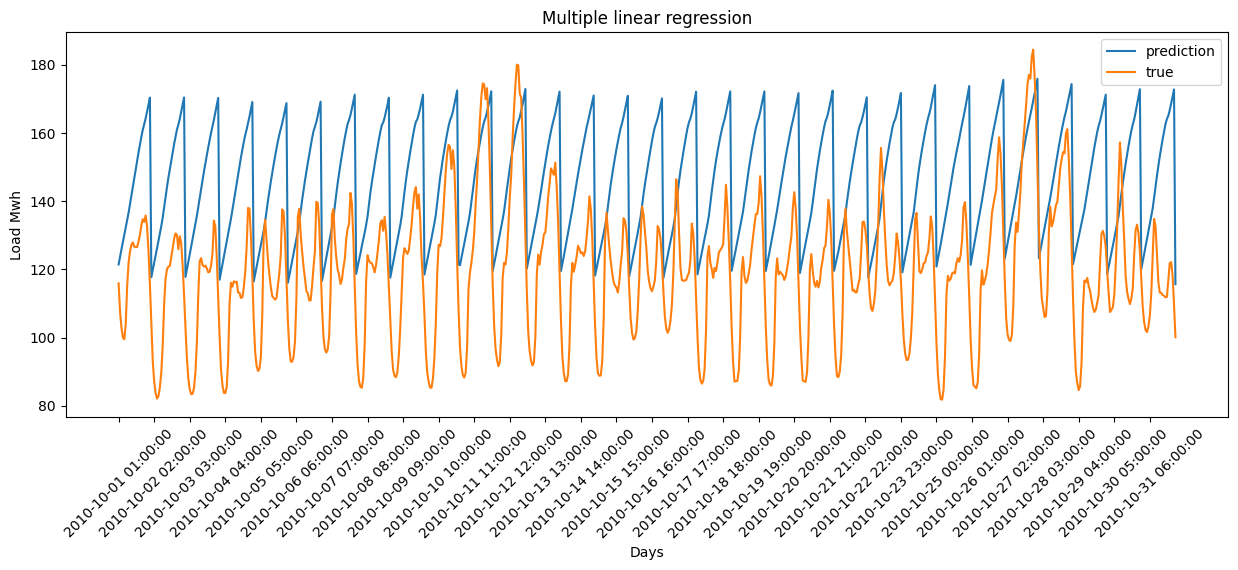
\includegraphics[width=\textwidth]{images/mlr_price.png}
    \caption{Multiple linear regression prediction}
    \label{fig:mlr_price}
\end{figure}

The resulting RMSE is 30.59.
What can be concluded, is that multiple linear regression is capable of catching the daily seasonality. Nevertheless, it cannot catch the range of the price series properly.

\subsection{Tbats}
Next, we tried with the autoregressive approach. Unfortunately, AR, ARIMA and SARIMA models did not perform as expected, their output was slightly better than the one of linear regression. This is probably due to the fact that, the data considered entails two kinds of seasonalities, while ARIMA models can only handle one at a time. We remind the reader, that the price time series involves both daily and weekly seasonalities. Hence, the need for a more advanced time series model. The Tbats model is a forecasting method capable of handling complex patterns in the data. Its name stands for trigonometric seasonality, Box-Cox transformation, ARMA errors, trend and seasonal components. 
Tbats forecast is visualized in figure \ref{fig:tbats_price}, meanwhile it RMSE is 15.08.
\begin{figure}[!h]
    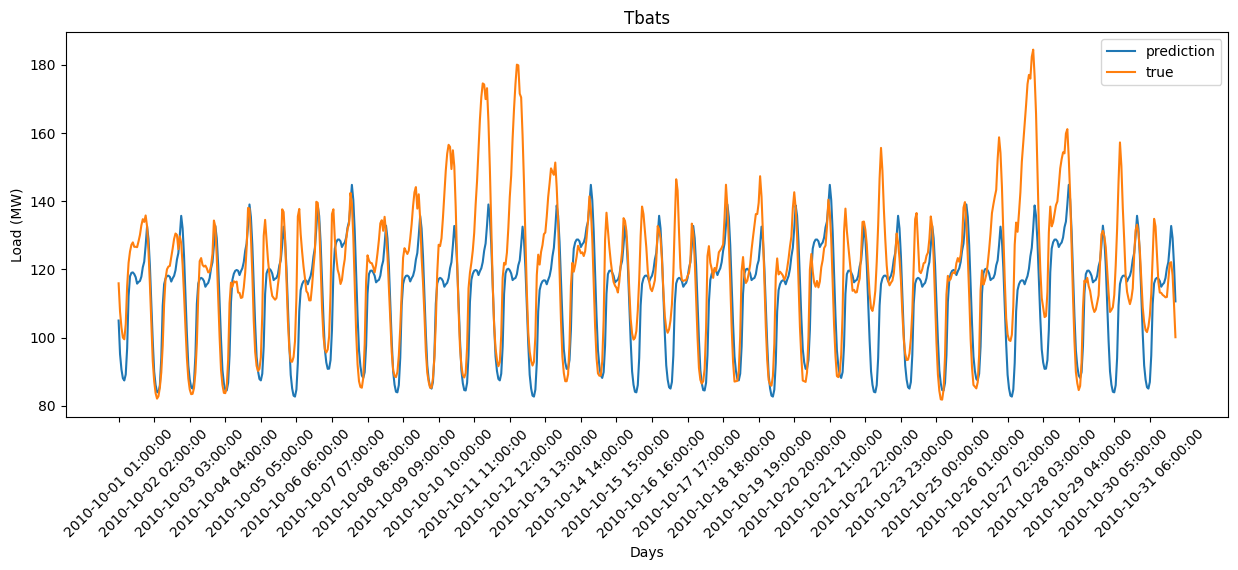
\includegraphics[width=\textwidth]{images/tbats_price.png}
    \caption{Tbats prediction}
    \label{fig:tbats_price}
\end{figure}
From the plot we see that Tbats is capable of catching the lows and average trend, conversely it has some difficulties handling the price peaks.
\subsection{Prophet}
Following, the prophet model has been considered. 
We get started by considering the base implementation. In such setting, prophet takes in as input the time series object and learns its data generating process.
This method achieves a RMSE of 23.96, its prediction is visualized in figure \ref{fig:prophet_price_1}.
\begin{figure}[!h]
    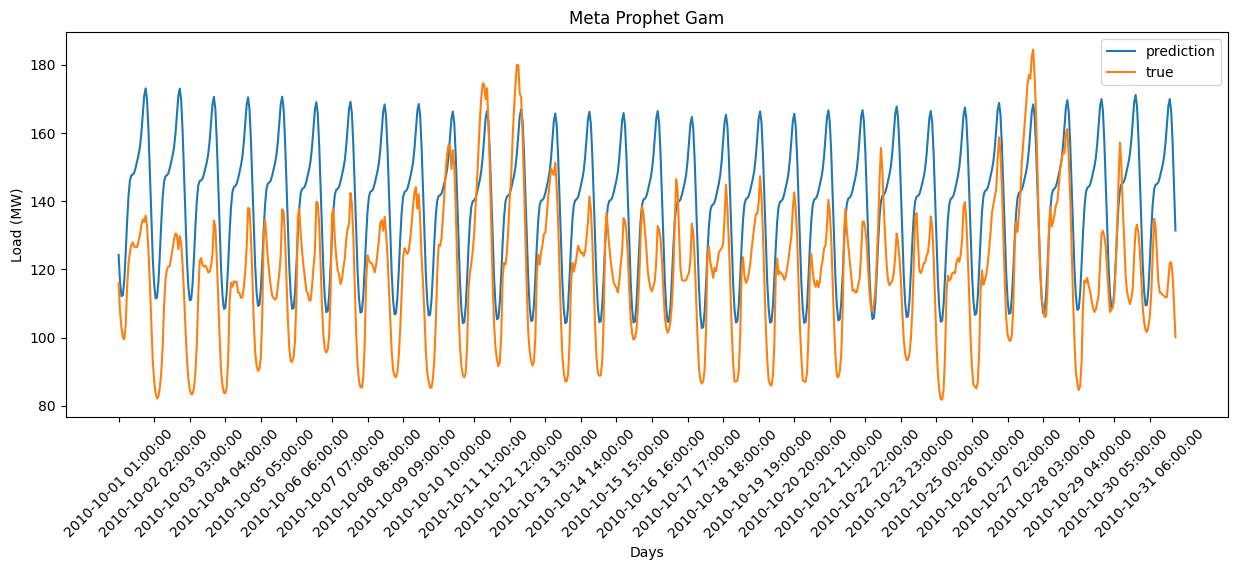
\includegraphics[width=\textwidth]{images/prophet_price_1.png}
    \caption{Prophet prediction}
    \label{fig:prophet_price_1}
\end{figure}
What can be seen is that, prophet models correctly the average trend but does not model peaks and lows precisely. 
Next, a more complex model was trained. We added the weather temperature, the square of it and the categorical variable for holidays effect as regressors. Furthermore, we also applied a log transformation to the dependet variable. Doing so, RMSE went down to 10.29. Forecast is visualized in \ref{fig:prophet_price2}, moreover, figure \ref{fig:prophet_price2.1} and figure \ref{fig:prophet_price2.2} break down the trend and the seasonalities respectively.
\begin{figure}[!h]
    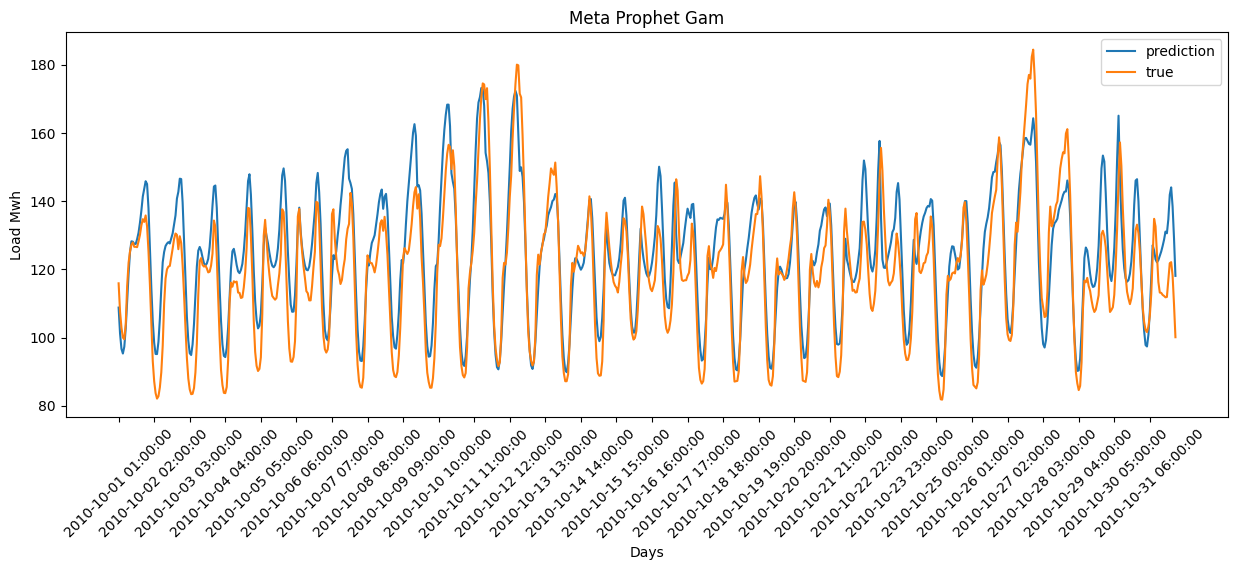
\includegraphics[width=\textwidth]{images/prophet_price2.png}
    \caption{Prophet v2 prediction}
    \label{fig:prophet_price2}
\end{figure}

\begin{figure}[!h]
    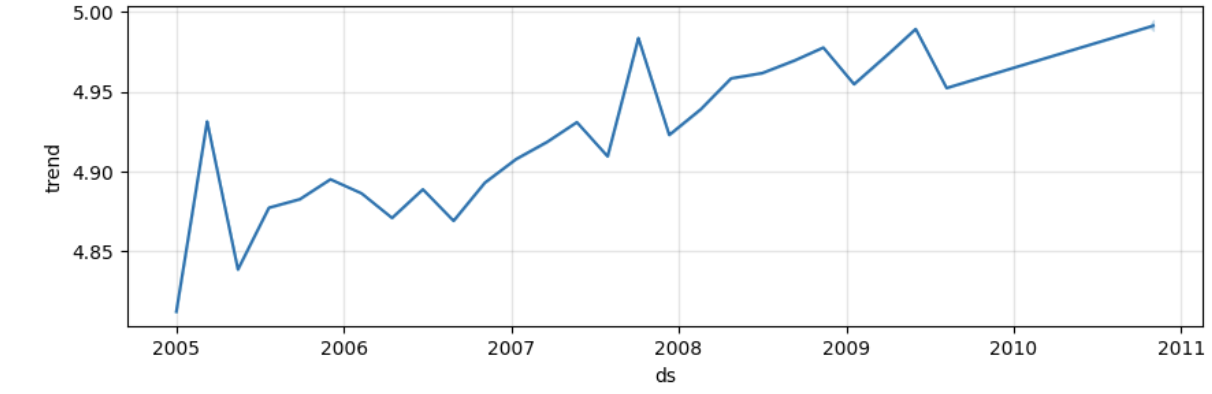
\includegraphics[width=\textwidth]{images/prophet_price2.1.png}
    \caption{Seasonalities breakdown}
    \label{fig:prophet_price2.1}
\end{figure}

\begin{figure}[!h]
    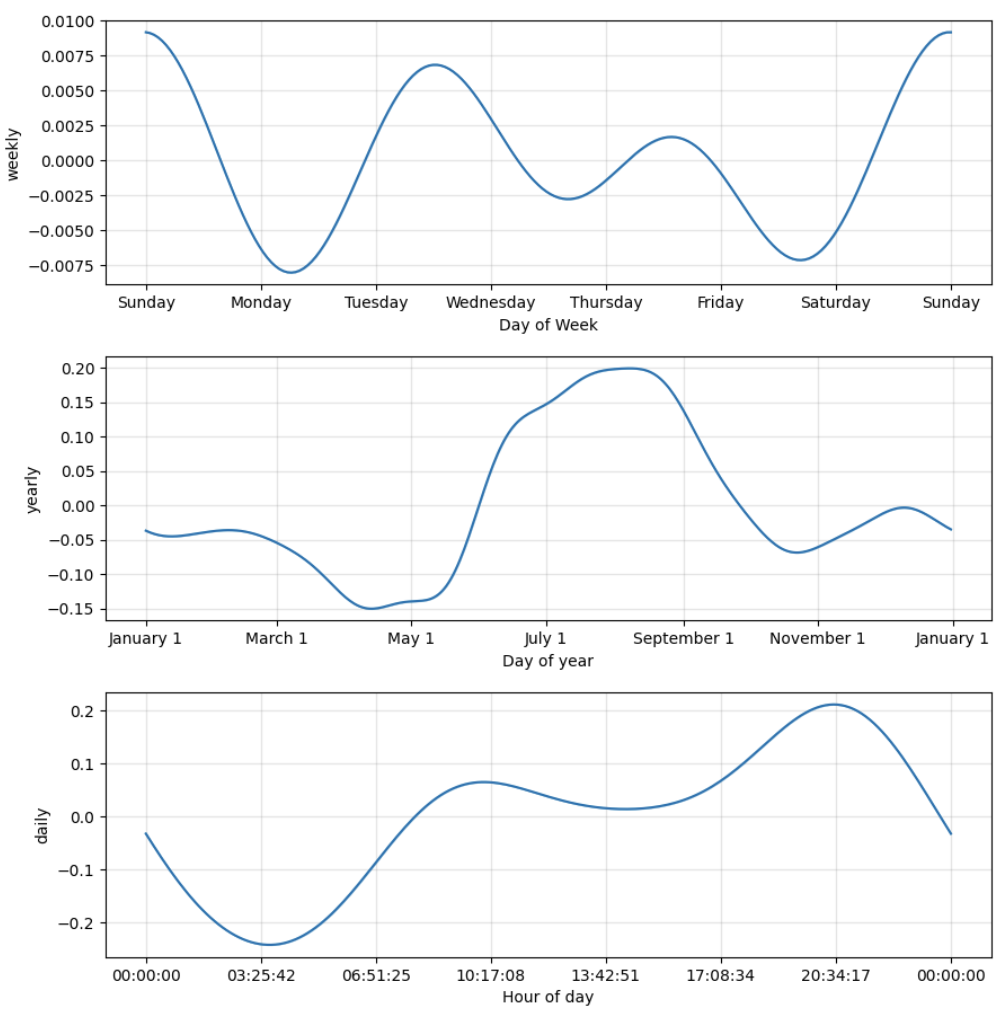
\includegraphics[width=\textwidth]{images/prophet_price2.2.png}
    \caption{Prices trend}
    \label{fig:prophet_price2.2}
\end{figure}
Prophet alongside with the right features is a good model in the context of electricity price forecasting, it is capcable of catching the trend, the peak and the lows. 

\subsection{K-nearest neighbours}
Afterwards, K-nearest neighbours has been considered. In doing so, we cross validated the number of neighbours to get the best model instance. The forecast is visualized in figure \ref{fig:knn_price}, RMSE is 12.54.
\begin{figure}[!h]
    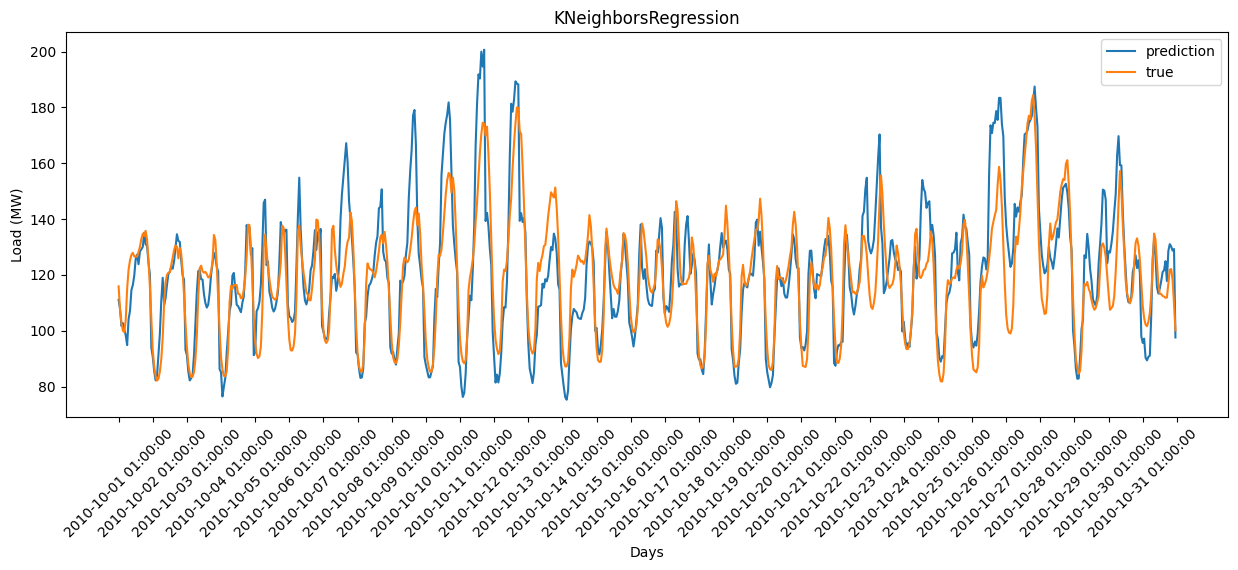
\includegraphics[width=\textwidth]{images/knn_price.png}
    \caption{K-nearest neighbour regression}
    \label{fig:knn_price}
\end{figure}
What it can be said is that, K-nearest neighbour is capable of predicting prices well by averaging past data.

\subsection{Support vector regression}
Coming up we have support vector regression. In applying this model we used gridsearch crossvalidation to search for the best regularization parameter C. Support vector regression achieves an RMSE of 23.24, for the prediction see figure \ref{fig:svr_price}.
\begin{figure}[!h]
    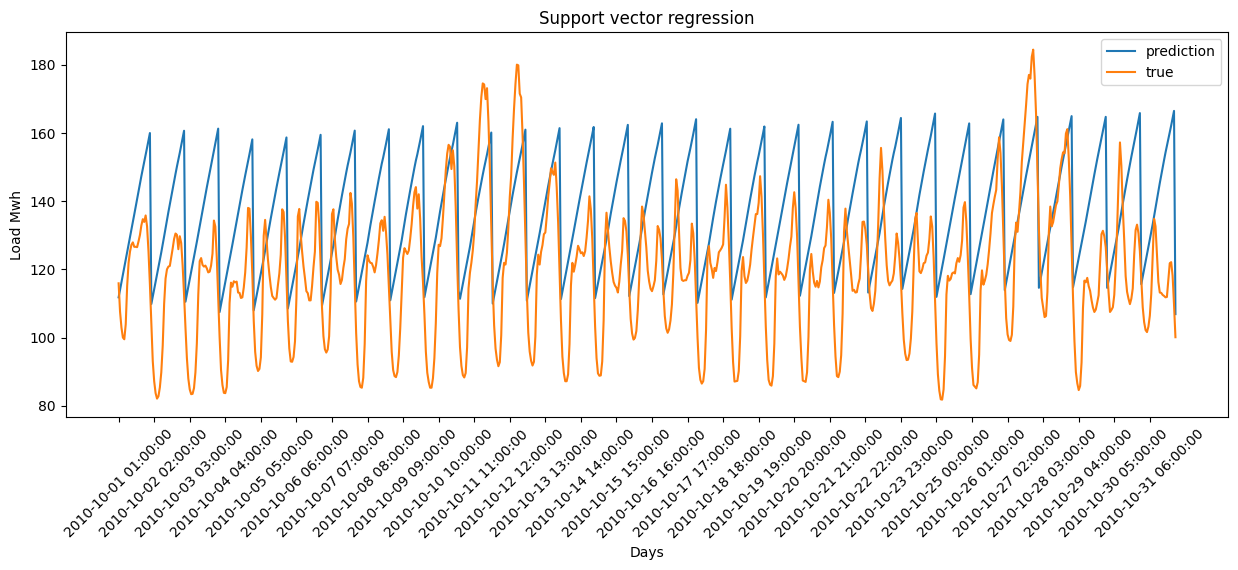
\includegraphics[width=\textwidth]{images/svr_price.png}
    \caption{Support vector regression prediction}
    \label{fig:svr_price}
\end{figure}
Visually, we see that the SVR performs similar to multiple linear regression as expected. Similarly to multiple linear regression, SVR can model the daily seasonality but the point prediction is off in terms of highs and lows.


\subsection{LSTM}

\subsection{Kernel ridge regression}
Subsequently, kernel ridge regression was considered. The kernel considered is the radial basis gaussian function.
Cross validation was carried jointly over the rbf kernel bandwith and the regularization constant.
The RMSE achieved is 9.86, figure \ref{fig:krnridge_price} reports the prediction.
\begin{figure}[!h]
    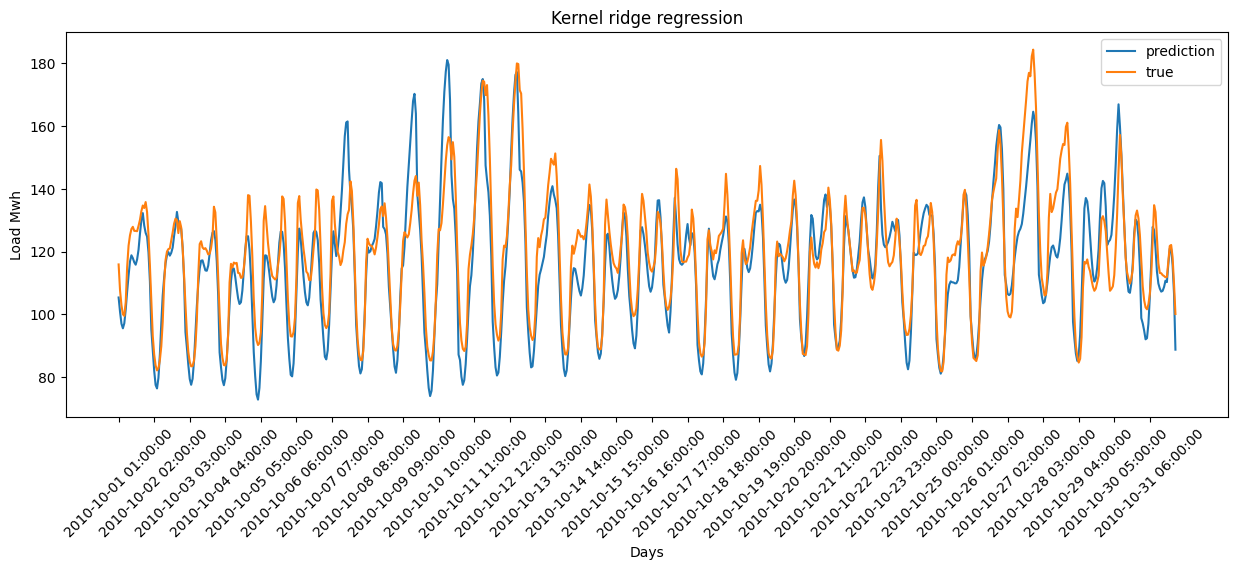
\includegraphics[width=\textwidth]{images/krnridge_price.png}
    \caption{Kernel ridge prediction}
    \label{fig:krnridge_price}
\end{figure}
We can observe that, kernel ridge regression models accurately the electricity time series.

\subsection{Kernel support vector regression}
The last model we considered in this setting was the kernel support vector regression.
RMSE achieved with this method is 9.10, forecast is reported in figure \ref{fig:krnsvr_price}.

\begin{figure}[!h]
    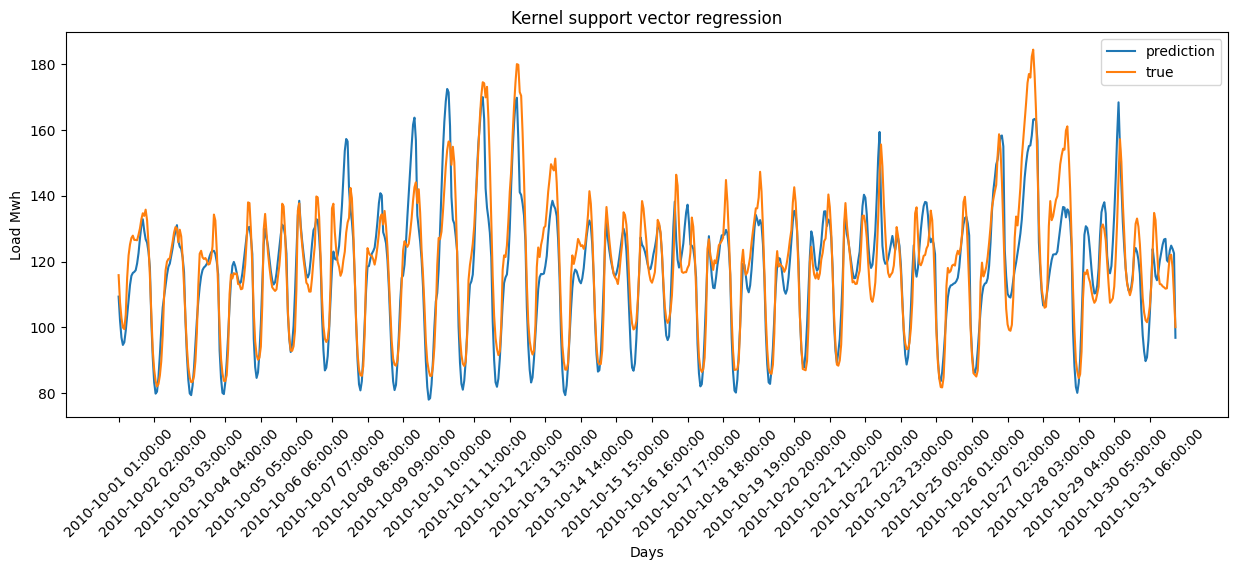
\includegraphics[width=\textwidth]{images/krnsvr_price.png}
    \caption{Kernel support vector prediction}
    \label{fig:krnsvr_price}
\end{figure}
We can observe that kernel support vector prediction is one of the best performing techniques between the one considered.


\subsection{Results}
This section reports the table comparing the considered methods in the context of electricity load forecasting.

- table 
|methods|tasks RMSE|
|       |X          |       
|       |X          |       

\section{Quantile forecasting}
In this subsection we compare performance of quantile regressor considering the GEFCom2014 dataset.
\\
- experiment for quantile estimator on gefcom2014 and we are good
